\documentclass{standalone}
\usepackage{tikz}
\usetikzlibrary{shapes.geometric}
\begin{document}
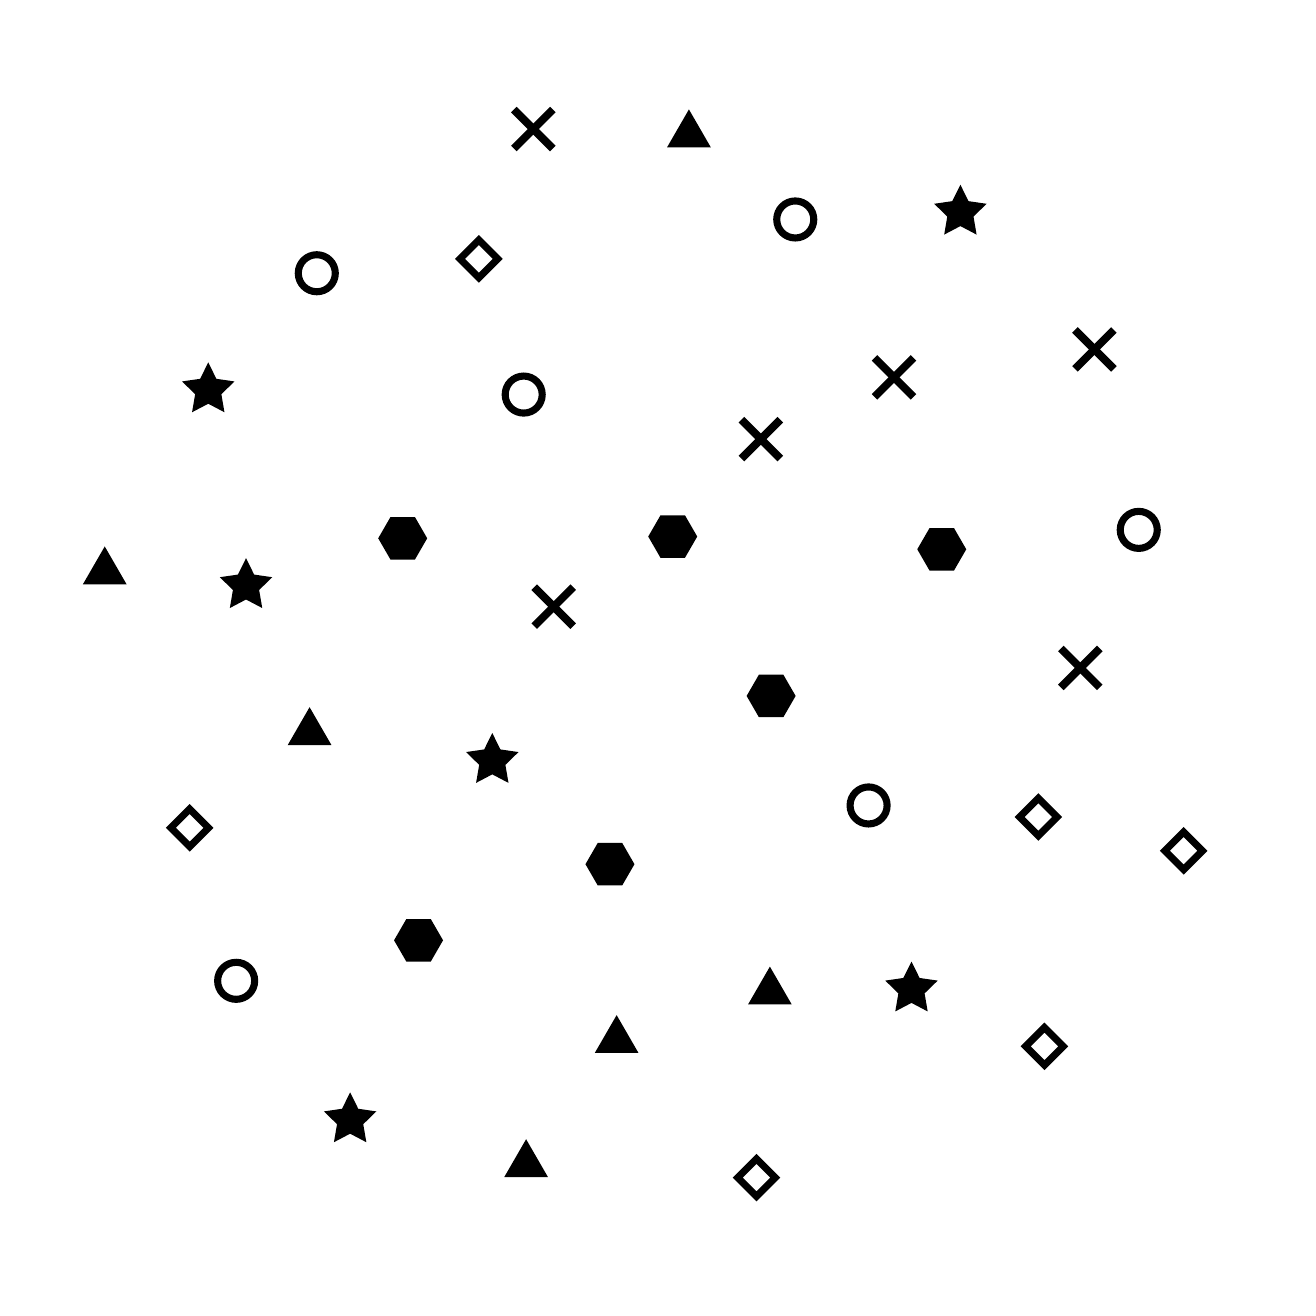
\begin{tikzpicture}
\node[circle,minimum width=160mm] at (0,0) {\phantom{1}};
\node[draw=black,circle,inner sep=1.875pt,line width=0.9mm] at (-5.35219,-4.10483) {\phantom{1}};
\node[draw=black,circle,inner sep=1.875pt,line width=0.9mm] at (-1.70045,3.34038) {\phantom{1}};
\node[draw=black,circle,inner sep=1.875pt,line width=0.9mm] at (1.74824,5.56416) {\phantom{1}};
\node[draw=black,circle,inner sep=1.875pt,line width=0.9mm] at (6.11053,1.62196) {\phantom{1}};
\node[draw=black,circle,inner sep=1.875pt,line width=0.9mm] at (-4.3282,4.88128) {\phantom{1}};
\node[draw=black,circle,inner sep=1.875pt,line width=0.9mm] at (2.67964,-1.8778) {\phantom{1}};
\node[text=black,rotate=45,inner sep=0pt] at (-1.57791,6.71269) {\rule{7mm}{1mm}};
\node[text=black,rotate=-45,inner sep=0pt] at (-1.57791,6.71269) {\rule{7mm}{1mm}};
\node[text=black,rotate=45,inner sep=0pt] at (1.31152,2.77456) {\rule{7mm}{1mm}};
\node[text=black,rotate=-45,inner sep=0pt] at (1.31152,2.77456) {\rule{7mm}{1mm}};
\node[text=black,rotate=45,inner sep=0pt] at (5.36811,-0.13142) {\rule{7mm}{1mm}};
\node[text=black,rotate=-45,inner sep=0pt] at (5.36811,-0.13142) {\rule{7mm}{1mm}};
\node[text=black,rotate=45,inner sep=0pt] at (5.54809,3.9133) {\rule{7mm}{1mm}};
\node[text=black,rotate=-45,inner sep=0pt] at (5.54809,3.9133) {\rule{7mm}{1mm}};
\node[text=black,rotate=45,inner sep=0pt] at (3.00269,3.55905) {\rule{7mm}{1mm}};
\node[text=black,rotate=-45,inner sep=0pt] at (3.00269,3.55905) {\rule{7mm}{1mm}};
\node[text=black,rotate=45,inner sep=0pt] at (-1.31947,0.64706) {\rule{7mm}{1mm}};
\node[text=black,rotate=-45,inner sep=0pt] at (-1.31947,0.64706) {\rule{7mm}{1mm}};
\node[regular polygon,regular polygon sides=3,fill=black,inner sep=0.0pt] at (-0.52008,-4.86064) {\phantom{1}};
\node[regular polygon,regular polygon sides=3,fill=black,inner sep=0.0pt] at (-7.02112,1.09118) {\phantom{1}};
\node[regular polygon,regular polygon sides=3,fill=black,inner sep=0.0pt] at (-1.66985,-6.43686) {\phantom{1}};
\node[regular polygon,regular polygon sides=3,fill=black,inner sep=0.0pt] at (0.39807,6.64145) {\phantom{1}};
\node[regular polygon,regular polygon sides=3,fill=black,inner sep=0.0pt] at (-4.41965,-0.95002) {\phantom{1}};
\node[regular polygon,regular polygon sides=3,fill=black,inner sep=0.0pt] at (1.42621,-4.24472) {\phantom{1}};
\node[draw=black,diamond,inner sep=0.8pt,line width=0.9mm] at (4.8361,-2.02455) {\phantom{1}};
\node[draw=black,diamond,inner sep=0.8pt,line width=0.9mm] at (1.25642,-6.604) {\phantom{1}};
\node[draw=black,diamond,inner sep=0.8pt,line width=0.9mm] at (6.68124,-2.45322) {\phantom{1}};
\node[draw=black,diamond,inner sep=0.8pt,line width=0.9mm] at (-2.26964,5.06375) {\phantom{1}};
\node[draw=black,diamond,inner sep=0.8pt,line width=0.9mm] at (-5.94278,-2.16183) {\phantom{1}};
\node[draw=black,diamond,inner sep=0.8pt,line width=0.9mm] at (4.91279,-4.93728) {\phantom{1}};
\node[star,star points=5,star point ratio=2,fill=black,inner sep=0.3pt] at (-3.90458,-5.8714) {\phantom{1}};
\node[star,star points=5,star point ratio=2,fill=black,inner sep=0.3pt] at (-5.22672,0.91271) {\phantom{1}};
\node[star,star points=5,star point ratio=2,fill=black,inner sep=0.3pt] at (-2.09935,-1.30789) {\phantom{1}};
\node[star,star points=5,star point ratio=2,fill=black,inner sep=0.3pt] at (-5.70652,3.39904) {\phantom{1}};
\node[star,star points=5,star point ratio=2,fill=black,inner sep=0.3pt] at (3.84555,5.65515) {\phantom{1}};
\node[star,star points=5,star point ratio=2,fill=black,inner sep=0.3pt] at (3.22435,-4.21031) {\phantom{1}};
\node[regular polygon,regular polygon sides=6,fill=black,inner sep=2.2pt] at (0.19227,1.53727) {\phantom{1}};
\node[regular polygon,regular polygon sides=6,fill=black,inner sep=2.2pt] at (1.44189,-0.487) {\phantom{1}};
\node[regular polygon,regular polygon sides=6,fill=black,inner sep=2.2pt] at (-0.60481,-2.62386) {\phantom{1}};
\node[regular polygon,regular polygon sides=6,fill=black,inner sep=2.2pt] at (3.60894,1.3753) {\phantom{1}};
\node[regular polygon,regular polygon sides=6,fill=black,inner sep=2.2pt] at (-3.03581,-3.59036) {\phantom{1}};
\node[regular polygon,regular polygon sides=6,fill=black,inner sep=2.2pt] at (-3.23703,1.51508) {\phantom{1}};
\end{tikzpicture}
\end{document}